\section{第三日第二讲}

\noindent{\small 记录人：Chun-Hsien Hsu、Weixiao Lu}

\medskip
我们此前提到应当有如下匹配：
\[
  \begin{array}{ccc}
    (M=TX) & & (\check M=T^*\check X)\\[2pt]
    G\curvearrowright X & & \check G\curvearrowright\check X\\[2pt]
    \Theta_G(X)\in A_G(Y) & \longleftrightarrow & \Theta_{\check G}(\check X)\in B_{\check G}(Y)
  \end{array}
\]
其中 $Y$ 取遍所有算术流形。本讲与下一讲的目标是把 $Y=\mathbb F_q((t))$ 这一情形的匹配解释清楚，办法是把 Plancherel 测度/Plancherel 公式几何化。我们将重写 Plancherel 测度，使两侧的配对看起来都像是某些 Hom 空间（被 q-特征标扭一下）；这将提示一个范畴等价，从而引出匹配的陈述/猜想。一旦得到匹配的陈述，我们再回过头来更深入地看 Plancherel 测度。

设 $F=\mathbb F_q((t))$，$O$ 是它的整数环。

\subsection{一个例子：$\mathbb G_m\backslash\mathrm{PGL}_2$}

我们先讨论 $X=\mathbb G_m\backslash\mathrm{PGL}_2$（右作用为 $G=\mathrm{PGL}_2$）的 Plancherel 测度，即昨天的第二个练习所考虑的情形。首先得弄清楚应当如何理解
\[
  X(F)/G(O)=F^\times\backslash\mathrm{PGL}_2(F)/\mathrm{PGL}_2(O).
\]
在上一讲我们见过 $\mathrm{PGL}_2(F)/\mathrm{PGL}_2(O)$ 可以画成一棵 $(q+1)$-正则树。现在我们换一种画法，以便容易描述 $F^\times$ 在树上的作用。取 $q=3$，于是画出的是一棵 $4$-正则树：

\begin{center}
  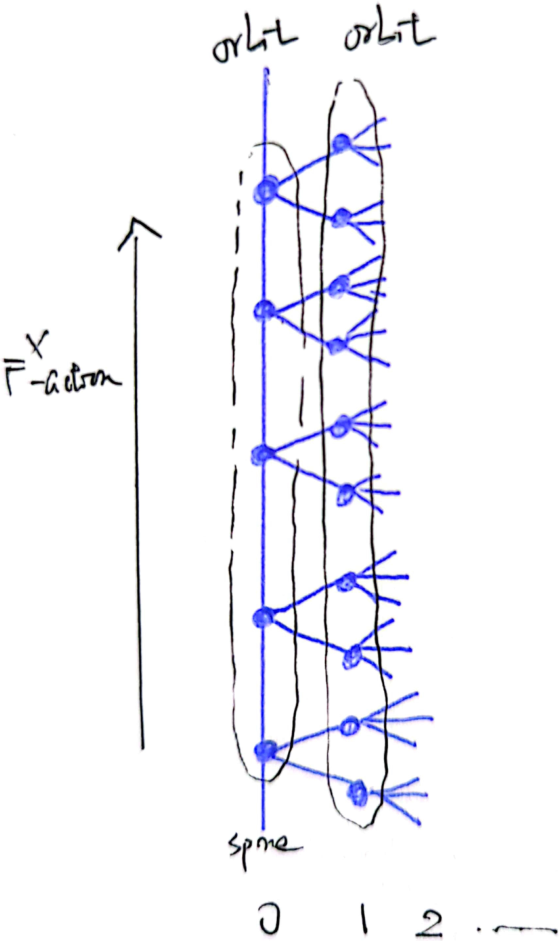
\includegraphics[width=0.33\textwidth]{figures/f91-spinetree.png}
\end{center}

于是 $F^\times$ 按竖直平移作用，而 $X(F)/G(O)$ 中的轨道由到 spine（轴）的距离给出，故
\[
  X(F)/G(O)\cong\mathbb Z_{\ge0}.
\]
因此可以像 $\mathrm{PGL}_2(O)\backslash\mathrm{PGL}_2(F)/\mathrm{PGL}_2(O)$ 的情形那样，把 Hecke 算子写成某些线性递推算子。最终在练习里你会证明
\begin{equation}
  \begin{array}{rcl}
    C_c^\infty(X(F))^{G(O)} & \xrightarrow{\ \sim\ } & \mathbb C[\mathrm{SL}_2/\mathrm{conj}]\\
    \text{基本函数}\ \delta_0=\mathbf 1_{X(O)} & \mapsto & 1\\
    \text{Hecke 算子} & \mapsto & \text{乘算子}\\
    \langle\cdot,\cdot\rangle & \leftrightarrow & \displaystyle\int_{\mathrm{SU}_2(\mathbb R)/\mathrm{conj}}|\cdot|^2\cdot(\check M=T^*\mathbb A^2\ \text{的 q-特征标})\,d_{Haar}.
  \end{array}
  \label{eq:9-1}
\end{equation}
注意 $\mathrm{SL}_2$ 是 $X$ 的对偶群（在此例中等于 $\mathrm{PGL}_2$ 的对偶群），而 $\mathrm{SU}_2=(\mathrm{SL}_2)_c$ 是 $\mathrm{SL}_2$ 的紧形式。稍后我们要做的是把内积与积分几何地重写为几何对象之间 Hom 空间的度量。

\subsection{历史}

不过在此之前，先谈谈匹配问题的历史。回忆对局部域 $F$，有 $A_G(F)=\Rep(G(F))$，而 $\Theta_G(X)=\mathrm{fns}(X(F))$ 是某种函数构成的表示，因此是 $G(F)$ 的表示，即 $\Theta_G(X)\in A_G(F)$。虽然一般局部域上表示论的研究是较晚的事，这类问题（研究 $\Theta_G(X)$ 如何落在 $A_G(F)$ 中）却被考虑了很长时间。

当 $F=\mathbb R$、Lie 群 $G$ 紧、$X$ 是紧 $G$-流形时，这可以追溯到 Cartan（1929）与 Weyl（1934）\footnote{Weyl, H. ``Harmonics on Homogeneous Manifolds.'' \emph{Annals of Mathematics}, vol.\ 35, no.\ 3, 1934, pp.\ 486--99.}。Weyl 与他的学生 Peter 用分析研究紧 Lie 群的表示。他们通过在 $G$ 上构造紧积分算子，证明了 $L^2(G)$ 可以分解为有限维不可约 $G$-表示的直和。后来 Cartan 证明，齐性 $G$-空间 $X$，
\begin{equation}
  L^2(X)\cong\bigoplus_\pi\pi^{m(\pi)},
  \label{eq:9-2}
\end{equation}
其中 $m(\pi)\in\mathbb Z_{\ge0}$ 是 $\pi$ 在 $L^2(X)$ 中的重数。

这个故事与另外两件事相关。第一，分解 (9.2) 与 $X$ 上微分算子的研究密切相关。例如对 $G=\mathrm{SO}_3$、$X=S^2$，这个分解对表示论学家与分析学家都是熟知的。因为它是按 Laplace 算子的本征空间作的分解；该分解给出球调和函数。更一般地，若 $D$ 是 $X$ 上与 $G$-作用交换的微分算子，则 $D$ 在 $L^2(X)$ 中的每个本征空间都是 $G$-表示。最理想的情形是所有重数都不超过 $1$，此时找本征函数与本征值最容易\footnote{而不是去解微分方程。}（由 Schur 引理，$D$ 在每个 $\pi$ 上作为标量作用）。此后许多推广都以此为目标。

与这个分解相关的另一件事是特殊函数的研究。Cartan 证明了当 $X$ 是紧 Riemann 对称空间时 $m(\pi)\le1$。为研究 $\pi$ 如何活在 $L^2(X)$ 中，他通过在 $X\times X$ 上构造 $G$-不变核（等价地，$(X\times X)/G$ 上的函数）来构造投影 $L^2(X)\to L^2(X)_\pi$（$\pi$ 的等类型部分），该核等于带球函数。这一观察很快就推广开了。特别地，到 60 年代 Vilenkin 写了一本书\footnote{Vilenkin, N.~Ja. \emph{Special functions and the theory of group representations}. Translated from the Russian by V.~N.~Singh. Translations of Mathematical Monographs, Vol.\ 22. American Mathematical Society, Providence, RI, 1968. x+613 pp.}，在更一般的设定下讨论此事，其中群 $G$ 不必紧，他研究两个 $G$-空间 $X$ 与 $Y$ 且 $L^2(X)_\pi\cong L^2(Y)_\pi\cong\pi$ 时的 $L^2(X)\to L^2(Y)_\pi$。此时核是 $(X\times Y)/G$ 上的函数。

他的观察是：推广这一进路，可以得到以表示为参数的各种特殊函数，并由此统一地恢复许多经典特殊函数，例如 Bessel 函数、超几何函数等等。

此后 Harish-Chandra 在 50 至 70 年代分类了实半单群 $G$ 的表示，并写出了群情形的 Plancherel 公式，即把 $L^2(G)$ 分解为 $G\times G$-表示，挑出基本函数 $\delta_e$（即 Dirac 测度），并弄清 $\delta_e$ 在分解中的去向。Harish-Chandra 的核心目标是 Plancherel 测度（即研究配对 $(L^2(G),\delta_e)$），而分类是在抵达目标的过程中得到的。从 60 到 70 年代起，人们开始考虑更一般空间的类似问题。其中一部分是研究双曲面上 Laplace 算子的分析学家。多数推广是在对称簇上做的。

2010 年前后，在 Sakellaridis--Venkatesh\footnote{Sakellaridis, Yiannis; Venkatesh, Akshay. \emph{Periods and harmonic analysis on spherical varieties}. Astérisque No.\ 396 (2017), viii+360 pp.} 中，我们提出：研究局部域上 $X$ 的 Plancherel 测度，是研究自守形式的 $X$-周期的局部类比。我们的书把调和分析与人们在自守形式上研究了很久的问题联系起来。与此前各情形一样，重数一假设\footnote{向量空间 $\Hom_G(C_c^\infty(X(F)),\pi)$ 对 $G(F)$ 的任一光滑不可约表示 $\pi$ 至多一维。}起特殊作用，这一点由 Piatetski-Shapiro 强调。这也是我们把范围限制在球簇（更精确地说，超球簇）上的主要原因，因为它们保证重数有限、有时还保证重数一。虽然 BZSV\footnote{D.~Ben-Zvi, Y.~Sakellaridis, A.~Venkatesh, \emph{Relative Langlands Duality}, preprint. 见 \url{https://www.math.ias.edu/~akshay/research/BZSVpaperV1.pdf}。} 非常代数，但手边有 $L^2$ 直觉有助于得到正确的归一化。

\subsection{设定}

假设 (9.1) 成立，并且为简单起见设 $\check G_X=\check G$。例如我们在 $(G,X,\check M)=(\mathrm{GL}_1,\mathbb A^1,T^*\mathbb A^1)$、$(\mathrm{PGL}_2,\mathrm{PGL}_2/\mathbb G_m,T^*\mathbb A^2)$ 见过这一点。

设 $V,W$ 是 $\check G$ 的有限维表示，$\chi_V,\chi_W$ 分别是 $V$ 与 $W$ 的特征标，$T_V,T_W$ 是 Satake 对应所联系的 Hecke 算子。我们要把恒等式
\[
  (T_V\delta_0,T_W\delta_0)=\int_{G^\vee_c}\chi_V(g)\chi_W(g)\cdot(\check M^\vee\ \text{的 q-特征标})\,d_{Haar}g
\]
的两端都几何地重写。左端将解释为 Frobenius 在某个对象 $?$ 上的迹，右端将解释为 q-作用（若 $q=1$ 就是维数）在另一个对象 $??$ 上的迹。这里 $?$ 与 $??$ 都是不同范畴中的 Hom 空间。这将引出我们关于范畴等价的猜想。
